\chapter{可见光多波段自适应通信系统硬件设计}
\section{引言}
我们在前面四章介绍了可见光通信的基本原理及关键技术,特别针对自适应传输这个核心重点研究了信道估计及比特功率分配算法,并且针对本课题对应的硬件平台的实际情况进行了别要的仿真,选出了合适的技术方案,如使用低复杂度的LS算法进行信道估计、使用高精度的EVM方法进行信噪比估计、使用专为可见光通信设计的Improved-SBLA比特功率分配算法得到自适应参数。本章将对可见光通信的硬件系统做一个简要的介绍,还将概述自适应模块的逻辑设计。
\section{硬件系统概述}
本课题对应的硬件演示平台如图\ref{fig:Hardware_Structure}所示,该系统目前已经实现了“编译级”的自适应传输,所谓“编译级”就是代码支持通过改变调制参数然后需要再编译来实现调制的改变,而真正的自适应传输系统因为时间紧迫及反向链路方案尚未确定等因素没有完成。不过本系统已有了自适应传输的雏形了,只是信道估计、计算自适应参数、改变调制等需要离线进行,下面对该系统进行概述。
\begin{figure}[htbp] 
\centering
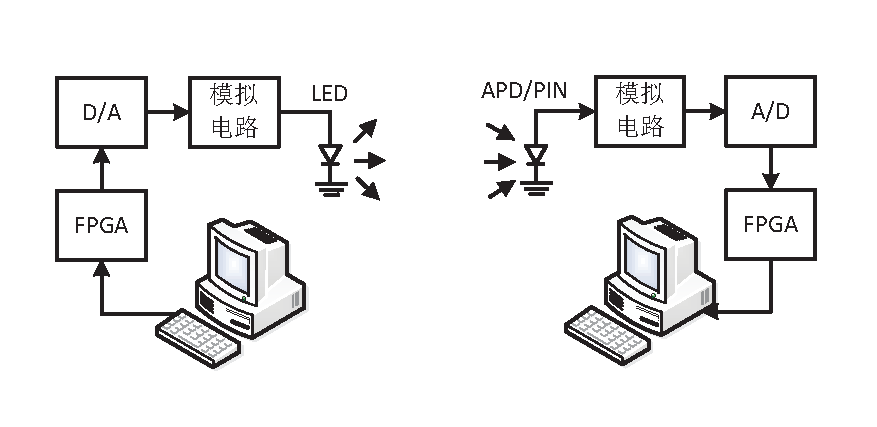
\includegraphics[width=0.8\textwidth]{figures/chapter-5/Hardware_Structure.eps}
\caption{可见光通信硬件平台示意图}
\label{fig:Hardware_Structure}
\end{figure}

首先信源比特通过以太网接口(UDP协议)按帧发送到用于基带处理的FPGA芯片(整个传输过程都是按帧进行的,并且用于同步和信道估计的ZC序列符号只在帧头处放置,整个帧中所有的OFDM符号都使用这个ZC序列估计出来的信道参数解调),接着在FPGA中完成扰码、信道编码、调制和IFFT等数字处理过程,然后将时域数字信号输入到数字模拟变换器(Digital to Analogue Converter,DAC)变成模拟信号,最后该模拟信号加上偏置电流之后去驱动LED灯,整个发射过程完成。接收端通过PD接收LED光信号,并将光信号强弱的变化转换成电信号的大小,然后将此模拟电信号送入模拟/数字变换器(Analog to Digital Converter,ADC)中抽样量化为数字信号,再送到接收端基带处理FPGA进行解调、解码和校验等操作,最后输出接收到的帧到接收端计算机。
\subsection{发射端基带处理}
发射端FPGA基带处理流程如图2所示,本演示系统信源帧长定为1358 byte(设置为该值主要是因为本系统主要以视频传输演示为主,而视频帧帧长就是1358 byte),为了系统设计简便起见,当通过以太网接口接到的帧不足1358 byte时,会自动在后面补零再传输。

基带处理芯片接收到信源帧之后,第一步就是对其加CRC,这里我们使用24 bit的循环校验码,循环校验比特的生成模块其实就是一个由生成多项式决定的除法电路,输入数据就是被除数,而余数就是我们需要的校验比特,当然为了加快计算速度,本系统CRC使用8位并行计算方法,即不是想真的除法电路那样逐比特地输入,而是一次输入8比特,整个运算速度提高了8倍。由于篇幅限制,在这里就不对CRC模块再进行过多的展开。得到24 bit(3 byte)校验位之后添加到原信源数据之后,又因为本系统使用的是输入为1362 byte的低密度奇偶校验码(Low Density Parity Code,LDPC)作为信道编码,所以1358 byte数据帧加入3 byte的校验码之后还要补零1 byte。为了防止过长的连0连1影响系统传输性能,所以还要把加了CRC及补零后的数据进行扰码再送入LDPC编码器。

信道编码是通过在发射数据中增加冗余以便在接收端可以进行信道解码纠错,本系统使用码率为3/4的LDPC码,输入数据长度为$1362\times 8$ bit,输出为14528 bit选择LDPC码的原因是其纠错性能佳,几乎适合所有信道,并且相对于Turbo码而言其解码器实现复杂度要低很多。这里使用的LDPC码的编码矩阵大小为$48\times 227$,所以输入数据位宽要为48 bit,而我们在CRC模块中输出数据位宽为8 bit,所以这里需要位宽变换,可以使用FPGA提供的RAM或先入先出队列(First In First Out,FIFO)数据结构来实现。编码之后的校验比特插在等间隔的插在信息数据中间,具体数据结构变化如下图所示。

经过编码的帧数据长度变为1816 byte,送入自适应调制模块,其功能是将信息比特分配到OFDM各个子载波上,并映射到星座图中的点,输出OFDM符号频域数据,这部分属于自适应设计的核心部分,将在下一节详细介绍。

经自适应模块调制后得到N个OFDM符号,N的值也调制的选择有关,假设根据自适应参数每个OFDM符号传输R比特,则有N=$\lceil 14528/\text{R} \rceil$,其中$\lceil \cdot \rceil$表示向上取整运算。为了提高传输速率,要保证所有的操作在一个OFDM帧周期内完成,所以要将将已调制符号交替存入两个RAM中,进行乒乓操作,即如果自适应模块再往其中RAM中写数据,则IFFT模块应该在另一个RAM中读数据去进行IFFT运算,到下一帧时这两个RAM的角色交换。IFFT模块可以使用Xilinx公司提供的IP核实现,并且可以通过设置自动添加添加循环前缀,非常方便。得到OFDM时域符号之后,在每帧的头部再加上ZC导频序列之后输入到DAC芯片输出,整个发射端基带处理就完成了。

\subsection{接收端基带处理}

\section{自适应模块FPGA方案设计}
\section{本章小结}